\section{Introduction}
Blockchain technology has revolutionized the way we create trustless and decentralized applications, offering immense composability and the ability to build complex primitives. This is particularly evident in the realm of decentralized finance (DeFi), where applications have been layered on top of each other to unlock new levels of functionality. However, the blockchain landscape is far from homogenous, with multiple blockchains employing different consensus protocols, varying assumptions of guaranteeing safety and liveness, and optimization for specific types of applications.

The challenge arises when we consider interoperability between these diverse blockchains. Composing applications on various chains is particularly challenging, as they struggle to interact seamlessly, resulting in fragmentation of user base and liquidity.

To address this issue, Cosmos\footnote{\url{https://cosmos.network}} has embraced the concept of ``The Internet of Blockchains''. In particular, it offers a modular blockchain stack that simplifies the creation of new blockchains via the Cosmos SDK. Cosmos chains can communicate and transact with each other through the Inter-Blockchain Protocol (IBC),\footnote{\url{https://ibcprotocol.dev}} enabling interoperability within the Cosmos ecosystem.

However, despite these strides which are to connect its own chains, a gap remains between the chains within and outside the Cosmos ecosystem. To bridge this divide, Axelar,\footnote{\url{https://axelar.network}} a Cosmos-based blockchain, has emerged as a solution, linking the Cosmos ecosystem to non-Cosmos chains, such as Ethereum, Bitcoin, Polygon, and others.

Ethereum, in particular, is one of the most widely used blockchains, hosting a multitude of decentralized applications spanning various sectors, including finance, gaming, and governance. Therefore, establishing a seamless and secure connection to Ethereum is of paramount importance for Axelar. By enabling interoperability with Ethereum, Axelar unlocks its rich ecosystem of decentralized applications and services.

This report focuses on methods of building a trustless connection between Axelar and Ethereum.

\subsection{Current Construction}
Currently, Axelar relies on a Tendermint-based delegated proof-of-stake consensus mechanism~\cite{axelar-whitepaper}. In particular, various validators lock stake, in the Axelar chain, and receive stake delegations from Axelar users. Following, the top $70$ validators, based on the aggregate (self and delegated) stake are chosen to participate in the Axelar consensus mechanism.

Axelar adopts a modular architecture to connect with different chains. Each connector module consists of two essential components. The first component verifies source chain (e.g., Ethereum) data into Axelar. The second component generates threshold signatures, which can be verified on the source chain. In this report, we focus exclusively on the former, that is verification of source chain data into Axelar.

Currently, connectors utilize an on-chain voting mechanism within Axelar to verify transactions that occurred on the source chain. Validators who vouch to participate in a connector attestation are referred to as \emph{attestors}. To determine the voting power of an attestor, Axelar employs quadratic voting. Briefly, the voting power of an attestor is the square root of their total stake. This mechanism aims to ensure a fair distribution of influence among attestors, based on their stake. To participate in the connector attestation, attestors are required to run a full node of the source chain and have access to the full node's RPC (Remote Procedure Call) interface. This enables attestors to verify the finalized transactions on the source chain, before voting for them on Axelar.

To initiate a bridge of data from the source chain to Axelar, a user interacts with an Axelar smart contract on the source chain. Subsequently, the user calls the corresponding connector module on Axelar, initiating the voting poll which is viewed by attestors. For each poll, an attestor decides whether to vote for or against it. To make an informed decision, the attestor queries the source chain's full node RPC and checks if the requested
transactions have been finalized on the source chain. If a poll receives sufficient attestations, it is accepted, otherwise it is rejected. 

This voting process forms the basis of verifying the source chain data into Axelar. 
Nonetheless, for the connector construction to function securely and maintain liveness, both the source chain and Axelar are assumed safe and live. In addition, the (quadratic) voting power distribution among the attestors is assumed to have an honest majority.

\subsection{Problem Statement}
The current construction of Axelar relies on attestors running the full node of the source chain to verify transactions and vote in an informed manner. However, this requirement imposes significant costs on attestors.\footnote{Indicatively, running a full Ethereum node requires $4+$ CPU cores, $16+$ GB RAM, at least $1$ TB SSD, and $25$ Mbps of stable connection (source: \url{https://www.quicknode.com/guides/infrastructure/node-setup/ethereum-full-node-vs-archive-node}).} 
Furthermore, as the Axelar network expands its support for additional chains, attestors will be required to run an increasing number of full nodes to verify transactions from these source chains.

This scalability bottleneck hampers the growth and efficiency of the Axelar network. Therefore, attestors are often incentivized to rely on third-party service providers to run and maintain the full nodes on their behalf. Unfortunately, the Axelar network lacks a mechanism to detect whether attestors are utilizing third-party providers or running the full nodes themselves --- in fact, it is unclear if such behavior is detectable.

This poses a significant centralization risk within the Axelar network. With a few dominant third-party providers in the market, attestors are likely to use the same service provider.\footnote{For example, at times $50$\% of Ethereum's transactions ran through one provider, Infura~\cite{infura}.} Consequently, if the third-party provider experiences a temporary compromise or breach, the entire Axelar network becomes vulnerable to attacks. The compromised provider could potentially censor transactions or even present incorrect transactions from the source chain to Axelar attestors, leading to financial losses for Axelar users.

In addition, collusion among attestors can also jeopardize Axelar's security. If an adversary gains a temporary majority over the quadratic voting power, particularly for (long-tail) chains with only a few attestors, the network becomes susceptible to attacks. 

In both situations outlined above, an honest Axelar validator who is not actively monitoring the source chain has no means to detect the attack and would accept incorrect data from it.

To address these challenges, we propose a construction that enables users or attestors to verify the consensus of the source chain within the Axelar execution layer. This is accomplished through light and super-light client constructions, in order to avoid relying on an honest majority among attestors.

In this report, we explore several constructions for light and super-light clients tailored specifically for Ethereum. We then propose a construction that best aligns with the requirements of Axelar, aiming to mitigate centralization risks, enhance security, and improve scalability.

\subsection{Preliminaries}
\noindent
\textbf{Execution model.}
A ledger protocol $\Pi$ is a distributed protocol that offers
a \emph{read} and \emph{write} functionality.
The ledger protocol is accompanied by a \emph{validity language}
$\mathbb{V}_{\Pi}$ containing all possible transactions that are ``legal''
according to the protocol $\Pi$.
The
\emph{read} functionality returns a \emph{ledger} in $\mathbb{V}_{\Pi}^*$,
whereas the \emph{write} functionality accepts a \emph{transaction} in $\mathbb{V}_\Pi$.
The \emph{ledger} is a finite sequence of pairs $(t, \tx)$ consisting
of an integer timestamp $t$ and a transaction $\tx$.

A particular protocol \emph{execution}
is one run of an environment $\mathcal{Z}_{\Pi,\mathcal{A}}$~\cite{uc} which simulates
the execution of $\Pi$ among multiple honest and adversarial parties. The adversarial
parties are controlled by one PPT adversary $\mathcal{A}$. The adversary and honest
parties are modelled as Interactive Turing Machines.
Out of the
$n_\Pi$ parties maintaining the ledger, $t_\Pi$ are corrupt and are controlled by the adversary
$\mathcal{A}$.

\noindent
\textbf{Networking.}
Time evolves in synchronous lock-step \emph{rounds} denoted by the integers $1, 2,
\ldots$. All parties have perfectly synchronized clocks, as they know the current round number.
Messages broadcast by an honest party at a round $r$ are received by all
other honest parties at the beginning of the next round $r + 1$. The adversary
can reorder messages, potentially different for each honest party,
inject different messages to the network tapes of different honest parties,
but cannot drop messages. We work in the \emph{client gossiping model} where
a new message received by any honest party is rebroadcast to all other honest
parties. We assume there are no bandwidth constraints.
The total execution time is polynomial, and each (honest or adversarial)
party is bound to polynomial time per round.

\noindent
\textbf{Sequence notation.}
In addition to its use to mean element-of-set, we will use $x \in A$ to mean that $x$
appears in the sequence $A$. We use $|A|$ for the length of the sequence $A$.
We write $A[i]$ for the $i$-th element of $A$ ($0$-based) and $A[-i]$ for the
$i$-th element of $A$ from the end. The element $A[-1]$ is the last element of $A$.
We denote by $A[{i}{:}{j}]$ the subarray of $A$ starting from element $i$ (inclusive)
and ending in element $j$ exclusive. The notation $A[{:}j]$ means the sequence
from the beginning up to $j$, whereas $A[i{:}]$ means the sequence from $i$ till
the end.

\noindent
\textbf{Ledgers.}
We denote $\Ledger[\Pi][P][r]$ the result of executing the \emph{read} functionality upon party $P$
operating in ledger protocol $\Pi$ at round $r$. The ledger $\Ledger[\Pi][P][r]$ of party $P$ at round $r$ is a sequence. We will write
$a \in S$ for an element $a$ and a sequence $S$ if the element $a$ appears somewhere in
the sequence $S$. For a ledger $L$ we will also use the notation $\tx \in L$ to mean that
the transaction $\tx$ appears in $L$ with some timestamp, that is, there exists some $t \in \mathbb{N}$
such that $(t, \tx) \in L$. In all practical blockchain-based ledger protocols, the timestamp $t$
associated with a transaction will correspond to the timestamp recorded on the block in which the
transaction is confirmed. As such, timestamps will all be in the past and non-decreasing.

A ledger protocol is \emph{safe} if the view of different honest parties is consistent.

\begin{definition}[Persistence]
  A ledger protocol $\Pi$ is \emph{persistent} during $I$ if for all honest parties $P_1, P_2$ at rounds
  $r_1, r_2 \in I$, with $r_1 < r_2$,
  we have that $\Ledger[\Pi][P_1][r_1] \preceq \Ledger[\Pi][P_2][r_2]$.
\end{definition}

A ledger protocol is \emph{live} if honest transactions make it to the ledger.

\begin{definition}[Liveness]
  A ledger protocol $\Pi$ is \emph{live} with liveness $u \in \mathbb{N}$ during $I$ if,
  for all honest parties $P_1, P_2$, whenever
  $P_1$ attempts to write a \emph{valid} transaction $\tx$ to the ledger at round $r \in I$,
  then for all $r' \in I$ with $r' \geq r + u$
  the transaction is included in $\Ledger[\Pi][P_2][r']$.
\end{definition}

\begin{definition}[Timeliness]
  A ledger protocol $\Pi$ is \emph{timely} with timeliness $\nu \in \mathbb{N}$ during $I$ if,
  for all honest parties $P$, and for all rounds $r$, it holds that:

  \begin{enumerate}
    \item $\Ledger[\Pi][P][r][-1]$ has a timestamp in the past, and
    \item $\Ledger[\Pi][P][r]$ has non-decreasing timestamps.
  \end{enumerate}

  Additionally, for all rounds $r \in I$, it holds that
  the timestamps recorded in $\Ledger[\Pi][P][r][|\Ledger[\Pi][P][r-1]|{:}]$
  are after $r - \nu$.
\end{definition}

Ledger security is defined as a ledger protocol that is both safe and live.

\begin{definition}[Security]
  A ledger protocol is \emph{secure} during $I$ with liveness $u$ if it is:

  \begin{enumerate}
    \item \emph{persistent} during $I$,
    \item \emph{live} with liveness $u$ during $I$, and
    \item \emph{timely} with timeliness $\tau$ during $I$.
  \end{enumerate}
\end{definition}

\noindent
\textbf{Bridges.}
A \emph{bridge} $\Lambda(\Pi_1, \Pi_2)$ is an interoperability protocol between two ledger protocols
$\Pi_1$ and $\Pi_2$. The execution is now one \emph{shared} environment $\mathcal{Z}$ between $\Pi_1$
and $\Pi_2$, but each of $\Pi_1$ and $\Pi_2$ are simulated internally by the environment exactly as before.
The purpose of the bridge is to relay events or information that take place on the source
side to the destination side. Without loss of generality, we consider $\Pi_1$ to be the \emph{source},
and $\Pi_2$ to be the \emph{destination}. If the bridge is bidirectional, our statements can be
applied in both directions. For our purposes, the purpose is to move value from one side to
the other.

A population of $n$ nodes, among which at most $t$ are adversarial, are responsible for operating the
bridge.

The bridge transmits certain transactions of interest from $\Pi_1$ to $\Pi_2$. These are \emph{cross-chain}
transactions and are defined by a function $\phi$ which accompanies the bridge protocol.

\begin{definition}[Cross-chain transaction]
  Let $\phi$ be an efficiently computable and invertible one-to-one
  injection $V_{\Pi_1} \longrightarrow V_{\Pi_2} \cup \{ \bot \}$.
  A transaction $\tx$ on the source side is a \emph{cross-chain} transaction if
  $\phi(\tx) \neq \bot$.
\end{definition}

Bridge liveness states that a transaction which appears on the source side will eventually make
it to the target side. Intuitively, this tells us that \emph{good things happen}. Whenever an
honest party attempts to cross the bridge, he will be successful in doing so.

\begin{figure}
    \center
    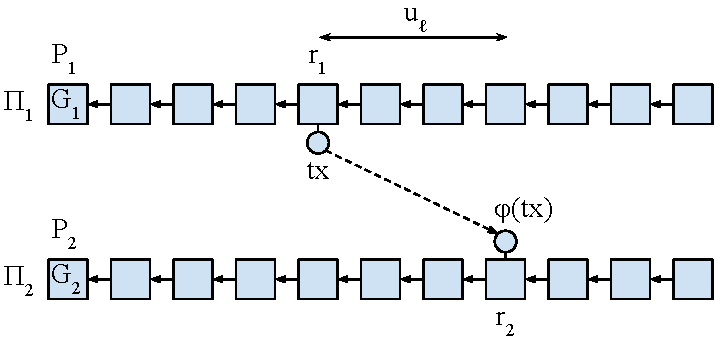
\includegraphics[width=0.7\columnwidth]{figures/bridge-liveness.pdf}
    \label{fig:bridge-liveness}
    \caption{Bridge liveness}
\end{figure}

\begin{definition}[Bridge Liveness]
  A bridge protocol $\Lambda(\Pi_1, \Pi_2)$ is \emph{live} with \emph{liveness} $u_\ell \in \mathbb{N}$
  during $I$ if, for all honest parties $P_1$ of $\Pi_1$ and $P_2$ of $\Pi_2$ and for all rounds
  $r_1, r_2 \in I$ with $r_2 \geq r_1 + u_\ell$ we have that, whenever $(t, \tx) \in \Ledger[\Pi_1][P_1][r_1]$
  with $t \in I$ and $\phi(\tx) \neq \bot$, then $\phi(\tx) \in \Ledger[\Pi_2][P_2][r_2]$.
\end{definition}

A visual depiction of bridge liveness is illustrated in Figure~\ref{fig:bridge-liveness}.
Even though our treatment is general to all ledger protocols and not particular to blockchains,
here we illustrate a blockchain example. A block containing $\tx$ appears in $\Pi_1$ in the view
of $P_1$ at round $r_1$. Soon after, in round $r_2 \leq r_1 + u\ell$, the corresponding transaction
$\phi(\tx)$ appears in the view of $P_2$ on $\Pi_2$.

Bridge safety mandates that a transaction appears on the destination side only if it has first
appeared on the source side, albeit with some delay. Intuitively, this tells us that \emph{bad
things don't happen}, because it's impossible for us to find a transaction paying out on the
destination without its preimage having appeared on the source. An adversary cannot make money
appear on the destination side without having paid on the source side.

\begin{figure}
    \center
    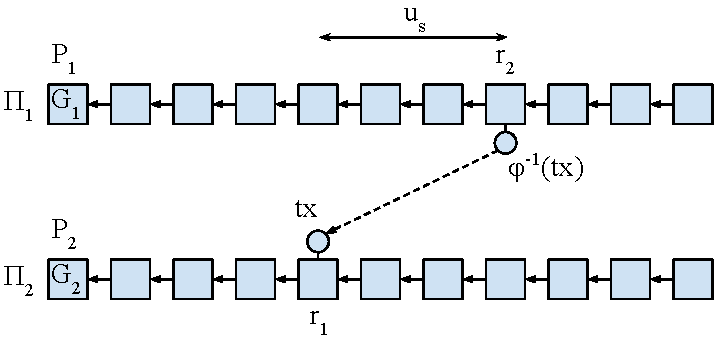
\includegraphics[width=0.8\columnwidth]{figures/bridge-safety.pdf}
    \label{fig:bridge-safety}
    \caption{Bridge safety}
\end{figure}

\begin{definition}[Bridge Safety]
  A bridge protocol $\Lambda(\Pi_1, \Pi_2)$ is \emph{safe} with \emph{safety} $u_s \in \mathbb{N}$
  during $I$ if, for all honest parties $P_1$ of $\Pi_1$ and $P_2$ of $\Pi_2$ and for all rounds
  $r_1, r_2 \in I$ with $r_2 \geq r_1 + u_s$ we have that, whenever $(t, \tx) \in \Ledger[\Pi_2][P_2][r_1]$
  with $t \in I$ and $\phi^{-1}(\tx) \neq \bot$, then
  $\phi^{-1}(\tx) \in \Ledger[\Pi_1][P_1][r_2]$.
\end{definition}

A visual depiction of bridge safety is illustrated in Figure~\ref{ref:bridge-safety}.
The party $P_2$ first observes the image $\tx$ on $\Pi_2$ at round $r_1$, and expects
another party $P_1$ to have already seen $\phi^{-1}(\tx)$ on $\Pi_1$. However, due to
network and consensus delays, this may be observed slightly later, but no later than at
round $r_2 \leq r_1 + u_s$.

\begin{definition}[Bridge Security]
  A bridge $\Lambda$ is \emph{secure} with safety $u_s \in \mathbb{N}$ and
  liveness $u_\ell \in \mathbb{N}$ during $I$ if it is safe with safety $u_s$ during $I$
  and live with liveness $u_\ell$ during $I$.
\end{definition} 

% - safety under dishonest majority in axelar network
% - healing 
% - incentives 
